\documentclass[11pt]{report}
\usepackage[utf8]{inputenc}
\usepackage[T1]{fontenc}
 \usepackage{listings}

\usepackage{fancyhdr}
\usepackage{graphicx}
\usepackage{color}
\pagestyle{fancy}


 \lhead{Geoffrey PERRIN - Océane DUBOIS}
 \rhead{}
 \rfoot{}



\definecolor{codegreen}{rgb}{0,0.6,0}
\definecolor{codegray}{rgb}{0.5,0.5,0.5}
\definecolor{codepurple}{rgb}{0.58,0,0.82}
\definecolor{backcolour}{rgb}{0.95,0.95,0.92}

\lstdefinestyle{mystyle}{
    backgroundcolor=\color{backcolour},
    commentstyle=\color{codegreen},
    keywordstyle=\color{magenta},
    numberstyle=\tiny\color{codegray},
    stringstyle=\color{codepurple},
    basicstyle=\footnotesize,
    breakatwhitespace=false,
    commentstyle=\color{codegreen},
    breaklines=true,
    captionpos=b,
    keepspaces=true,
    numbers=left,
    numbersep=5pt,
    showspaces=false,
    showstringspaces=false,
    showtabs=false,
    tabsize=2,
     morekeywords={mov, push, xor, extern, div, mov, inc, cmp, jne, call, pop, ret,endp, proc, end, dec, add, jb, dd, db, jge,  not, lea, main, public, movzx},
   extendedchars=true,
    sensitive=false,
   morecomment=[l]*,
   morecomment=[l];,
    literate= {á}{{\'a}}1 {é}{{\'e}}1 {í}{{\'i}}1 {ó}{{\'o}}1 {ú}{{\'u}}1 {Á}{{\'A}}1 {É}{{\'E}}1 {Í}{{\'I}}1 {Ó}{{\'O}}1 {Ú}{{\'U}}1 {à}{{\`a}}1 {è}{{\`e}}1 {ì}{{\`i}}1 {ò}{{\`o}}1 {ù}{{\`u}}1 {À}{{\`A}}1 {È}{{\'E}}1 {Ì}{{\`I}}1 {Ò}{{\`O}}1 {Ù}{{\`U}}1 {ä}{{\"a}}1 {ë}{{\"e}}1 {ï}{{\"i}}1 {ö}{{\"o}}1 {ü}{{\"u}}1 {Ä}{{\"A}}1 {Ë}{{\"E}}1 {Ï}{{\"I}}1 {Ö}{{\"O}}1 {Ü}{{\"U}}1 {â}{{\^a}}1 {ê}{{\^e}}1 {î}{{\^i}}1 {ô}{{\^o}}1 {û}{{\^u}}1 {Â}{{\^A}}1 {Ê}{{\^E}}1 {Î}{{\^I}}1 {Ô}{{\^O}}1 {Û}{{\^U}}1,
  }

\lstset{style=mystyle}

%Gummi|065|=)
\title{\textbf{TP05 - Traitement d'image - première partie }
\author{Geoffrey PERRIN \\ Océane DUBOIS\\}
\date{}}

\begin{document}

\maketitle

\newpage

\section{squelette du sous-programme process\_image\_asm}

Sachant que le compilateur empile les arguments dans l'ordre inverse de celui dans lequel ils sont passés à la fonction, ecx contient d'abord la largeur de l'image puis il est multiplié par la hauteur de l'image, ainsi on obtient le nombre de pixels de l'image.
Dans esi, on met le pointeur vers l'image source et edi contient un pointeur vers l'image tempon 1.


\begin{figure}[ht]
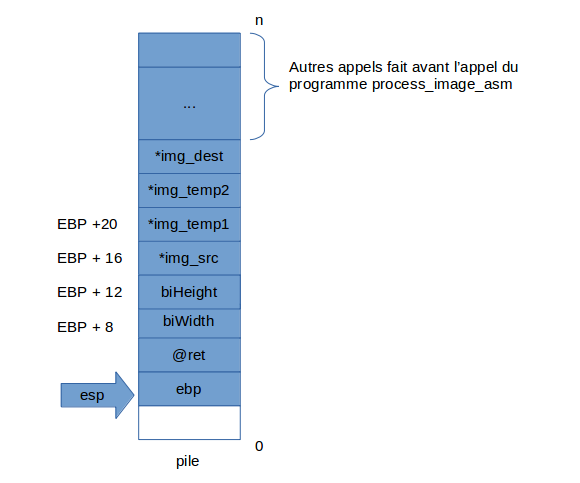
\includegraphics[width=8cm]{pile.png}
\caption{Etat de la pile juste après l'appel de process\_image\_asm}
\end{figure}

\section{Conversion en niveaux de gris}

Sachant que les pixels sont indexés de 1 à n, et que ecx contient l'index d'un pixel donné et esi contient un pointeur vers l'image source, on peut exprimer edi ainsi : $edi=esi+ecx*4-1$
En effet on ajoute au pointeur de l'image de départ, l'index du pixel multiplié par 4 qui correpond à la taille d'un pixel (un pixel occupe 4 octets en mémoire) et on retire 1 car les pixels sont indexés de 1 à n.


Pour parcourir tous les pixels de l'image source, on utilise une structure de type :
\begin{lstlisting}
do{
	traitement de l'image;
	ecx - -;
}while(ecx >=0);
\end{lstlisting}
\medskip

En assembleur cela correspond à :


//// METTRE LE CODE ASSEMBLEUR QU'ON A UTILISE POUR LE WHILE


Il est plus facile de partir du dernier pixel de l'image car ecx contient déjà le nombre de pixel total de la photo.

Pour convertir une image en nuance de gris on utilise la formule suivante :
$I=R*0,299+V*0,587+B*0,114$

On converti pour la suite du TP les coefficients de ce calcul en hexadécimal.
On obtient donc, en virgule fixe sur 16 bits avec un décalage à la virgule de +8 :
\begin{itemize}
\item  Cr = 0,299 =  00,4Ch
\item  Cv = 0,587 = 00,96h
\item  Cb = 0,114 = 00,1Dh
\end{itemize}

/////EXPLIQUER COMMENT MULTIPLIER DEUX NOMBRES DE 16 BITS AVEC VIRGULE FIXE

Pour faciliter le calcul sachant que la partie entiere des coefficient et que la partie décimal des valeur de RVB sont toujours nulle on peut simplifier le calcul:

On décale de 8 bits a gauche les coefficients. (On peut se permmetre de perdre l'information de la partie entiere car elle est toujours nulle.)
Alors Cr = 4Ch, Cv = 96h, Cb=1Dh.
Ainsi les coefficients sont réduit a des entiers de 8 bits.

De plus la partie décimal des valeurs de R,V,B étant nulle on peut réduire ces valeurs a des entier de 8 bit en ométant la partie décimal.

On a donc transformé la multiplication entre deux réels de 16 bits en une multiplication entre deux entiers de 8 bits.

Mais en faisant ce décalage de 8 bits vers la gauche on a multiplié le resultat final par 256.
Il suffit donc de redécaler de 8 bits vers la droite le résultat final pour le diviser par 256 et donc trouver le résultat attendu.


Lors de la conversion des coefficient en hexadecimal sur 16 bits nous ne faisons qu'approcher la valeur des coefficient. Il y a une perte d'informaton lié au nombre limité de bit.

Sachant que la valeur max que peut prendre les coefficients R, V et B est 255 et que la somme des 3 coefficient du calcul de I est inférieur ou égale 1, on aura donc comme valeur max $1*255$, qui vaut donc 255. Sur 8 bits on peut coder au plus 255 valeurs, il n'y aura donc pas de débordements.
Nous avons décidé d'arrondir au coefficient inferieur le plus proche pour que la somme des coeffcients reste inferireur ou égale a 1.

On souhaite éviter les débordements pour éviter de perdre de l'information sur l'image.

\medskip

/// METTRE LE CODE ASSEMBLEUR EN CONSIDERANT QUE R, V, et B SONT DES ENTIERS A VIRGULE



On peut effectivement simplifier l'algorithme en considérant qu la partie entière des coefficients multiplicateurs est toujours nulle et que la partie décimales des coefficient R, V, B est toujours nulle.

Voici donc le code avec la simplification, on stockera l'image dans l'image temporaire 1 : 



//FAIRE DES TEST SUR LA VITESSE D'EXECUTION DU PROGRAMME EN C ET EN ASSEMBLEUR
\end{document}
